%-*-latex-*-
%-*-latex-*-
\newcommand\COURSE{ciss245}
\newcommand\ASSESSMENT{q05}
\newcommand\ASSESSMENTTYPE{Quiz}
\newcommand\POINTS{\textwhite{xxx/xxx}}

\makeatletter
\DeclareOldFontCommand{\rm}{\normalfont\rmfamily}{\mathrm}
\DeclareOldFontCommand{\sf}{\normalfont\sffamily}{\mathsf}
\DeclareOldFontCommand{\tt}{\normalfont\ttfamily}{\mathtt}
\DeclareOldFontCommand{\bf}{\normalfont\bfseries}{\mathbf}
\DeclareOldFontCommand{\it}{\normalfont\itshape}{\mathit}
\DeclareOldFontCommand{\sl}{\normalfont\slshape}{\@nomath\sl}
\DeclareOldFontCommand{\sc}{\normalfont\scshape}{\@nomath\sc}
\makeatother

\input{myquizpreamble}
\input{yliow}
\input{\COURSE}
\textwidth=6in

\renewcommand\TITLE{\ASSESSMENTTYPE \ \ASSESSMENT}

\newcommand\topmattertwo{
\topmatter
\score \\ \\
Open \texttt{main.tex} and enter answers (look for
\texttt{answercode}, \texttt{answerbox}, \texttt{answerlong}).
Turn the page for detailed instructions.
To rebuild and view pdf, in bash shell execute \texttt{make}.
To build a gzip-tar file, in bash shell execute \texttt{make s} and
you'll get \texttt{submit.tar.gz}.
}

\newcommand\tf{T or F or M}
\newcommand\answerbox[1]{\textbox{\phantom{|}\hspace{-4mm}#1}}
\newcommand\codebox[1]{\begin{console}#1\end{console}}

\usepackage{pifont}
\newcommand{\cmark}{\textred{\ding{51}}}
\newcommand{\xmark}{\textred{\ding{55}}}

\newcounter{qc}
\newcommand\nextq{
%\newpage
\addtocounter{qc}{1}
Q{\theqc}.
}

\DefineVerbatimEnvironment%
 {answercode}{Verbatim}
 {frame=single,fontsize=\footnotesize}

\newenvironment{largebox}[1]{%
 \boxparone{#1}
}
{}

\usepackage{environ}
\let\oldquote=\quote
\let\endoldquote=\endquote
\let\quote\relax
\let\endquote\relax

% ADDED 2021/09/09
\renewcommand\boxpar[1]{
 \[
  \framebox[\textwidth][c] {
   \parbox[]{\dimexpr\textwidth - 0.25cm} {#1}
  }
 \]
}

\NewEnviron{answerlong}%
  {\vspace{-1mm} \global\let\tmp\BODY\aftergroup\doboxpar}

\newcommand\doboxpar{%
  \let\quote=\oldquote
  \let\endquote=\endoldquote
  \boxpar{\tmp}
}

\newenvironment{mcq}[7]%
{% begin code
#1 \dotfill{#2}
 \begin{tightlist}
 \item[(A)] #3
 \item[(B)] #4
 \item[(C)] #5
 \item[(D)] #6
 \item[(E)] #7 
 \end{tightlist}
}%
{% end code
} 

\renewcommand\EMAIL{}
\newcommand\score{%
\vspace{-0.6in}
\begin{flushright}
Score: \answerbox{\POINTS}
\end{flushright}
\vspace{-0.4in}
\hspace{0.7in}\AUTHOR
\vspace{0.2in}
}

\newcommand\blankline{\mbox{}\\ }


\renewcommand\AUTHOR{crsmith14@cougars.ccis.edu} % CHANGE TO YOURS

\begin{document}
\topmattertwo

%-*-latex-*-
\textsc{Instructions}
\begin{enumerate}
\li This is a closed-book, no-discussion, no-calculator, no-browsing-on-the-web
    no-compiler/no-MIPS-simulator test.
\li Cheating is a serious academic offense. If caught you will 
    receive an immediate score of -100\%.
\li If a question asks for a program output and the program or
    code fragment contains
    an error, write \verb!ERROR! as output.
    When writing output, whitespace is significant.
\li If a question asks for the computation of a value and the program or
    code fragment contains
    an error, write \verb!ERROR! as value.
\li When you're asked to write a C++ statement, don't forget that it must
    end with a semicolon.
\li Bubblesort refers to the bubblesort algorithm in our notes
    where values are sorted in ascending order.
\end{enumerate}

\vspace{1cm}


\begin{center}
  \textsc{Honor Statement}
\end{center}
I, \answerbox{Corban Rei Smith},
attest to the fact that the submitted work is my own and
is not the result of plagiarism.
Furthermore, I have not aided another student in the act of
plagiarism.

% ------------------------------------------------------------------------------
\begin{python}
from scoretable import *
\end{python}
        
%-------------------------------------------------------------------------------
\newpage
\nextq
Complete the following program. You can only add to the given code.
You cannot delete or change what is given below.

\textsc{Answer:}
\begin{answercode}
#include <iostream>

void swap(int * p, int * q)
{
  int t = *p;
  *p = *q;
  *q = t;
}


int main()
{
    int x = 0;
    int y = 1;

    swap(&x,&y);
    
    std::cout << x << ' ' << y << '\n'; // expected output: 1 0
    
    return 0;
}
\end{answercode}

% ------------------------------------------------------------------------------
\newpage
\nextq
Complete the following program.
You can only add to the given code. 
You cannot delete or change what is given below.

The function \verb!reverse(x, x_len)! reverses the values in the integer
array \verb!x!
from index \verb!0! up to index \verb!x_len - 1!.
For instance suppose the user enters \verb!2 3 5 7 -9999!, then
the values \verb!2, 3, 5, 7! are placed in \verb!x!
and \verb!x_len! is set to 4.
After calling \verb!reverse(x, x_len)!,
the first four value in \verb!x! becomes \verb!7, 5, 3, 2!.

\textsc{Answer:}
\begin{answercode}
#include <iostream>

void reverse(int x[], int x_len)
{

  for (int i = x[] - 2; i >= 0; --i)
  {
    for (int j = 0; j <= i; ++j)
    {
      if (x[j] > x[j + 1])
      {
        int t = x[j]; x[j] = x[j + 1]; x[j + 1] = t;
      }
    }

}


int main()
{
    int x[1024];
    int x_len;

    x_len = 0;
    for (int i = 0; i < 1024; ++i)
    {
        int t;
        std::cin >> t;
        if (t == -9999)
        {
            break;
        }
        x[x_len] = t;
        ++x_len;
    }

    reverse(x, x_len);
    // x from index 0 to x_len - 1 is now reverse.
    
    return 0;
}
\end{answercode}

% ------------------------------------------------------------------------------
\newpage
\nextq
What is the output of this program?
\begin{Verbatim}[frame=single]
int x = 10;
int y = 20;
int * p = &x;
int * q = &y;
*p = *p * *q;
*q = 42;
std::cout << x << ' ' << y << '\n';
std::cout << *p << ' ' << *q << '\n';
\end{Verbatim}

\textsc{Answer:}
\begin{answercode}
200 42
200 42
\end{answercode}

%-------------------------------------------------------------------------------
\newpage
\nextq
Rewrite the following code fragment by doing the following: Do a simple addition
program using the following skeleton.
You MUST follow the given instructions.

\textsc{Answer:}
\begin{answercode}
int x = 0, y = 0;
int * p = &x;
int * q = &y;
// Do NOT declare any variables below.

// Statement to get an integer from user and put it into x.
// Do NOT use x in your statement.
std::cin >> *p;



// Statement to get an integer from user and put it into y.
// Do NOT use y in your statement.
std::cin >> *q;



std::cout << x + y << '\n';
\end{answercode}

%-------------------------------------------------------------------------------
\newpage
\nextq
What is the output of this code fragment?
\begin{Verbatim}[frame=single]
int i = 1;
int j = 2;
int k = 3;
int * p = &i;
int * q = &j;
int * r = &k;
p = q;
q = r;
std::cout << *p << ' ' << *q << ' ' << *r << '\n'; 
\end{Verbatim}

\textsc{Answer:}
\begin{answercode}
2 3 3

\end{answercode}

%-------------------------------------------------------------------------------
\newpage
\nextq
You were brainstorming with your team in one of the company's meeting rooms.
Your boss popped in to say hi on his way to get coffee and
he noticed the following diagram on the whiteboard.
Someone was tracing a piece of code on the whiteboard:
\begin{center}
  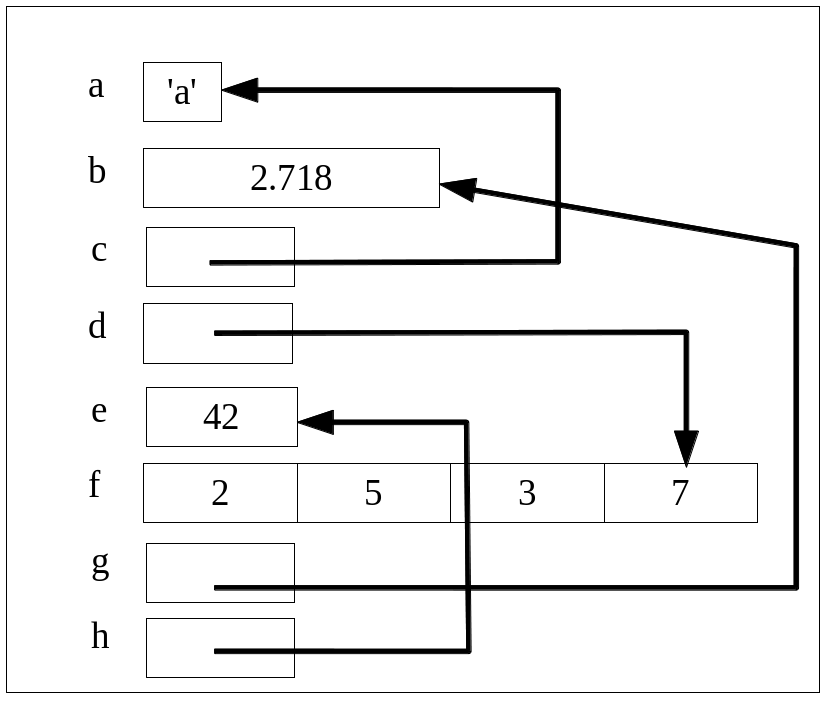
\includegraphics[width=3in]{pic1.PNG}
\end{center}
On his way back, your boss glanced at the whiteboard and saw this:
\begin{center}
  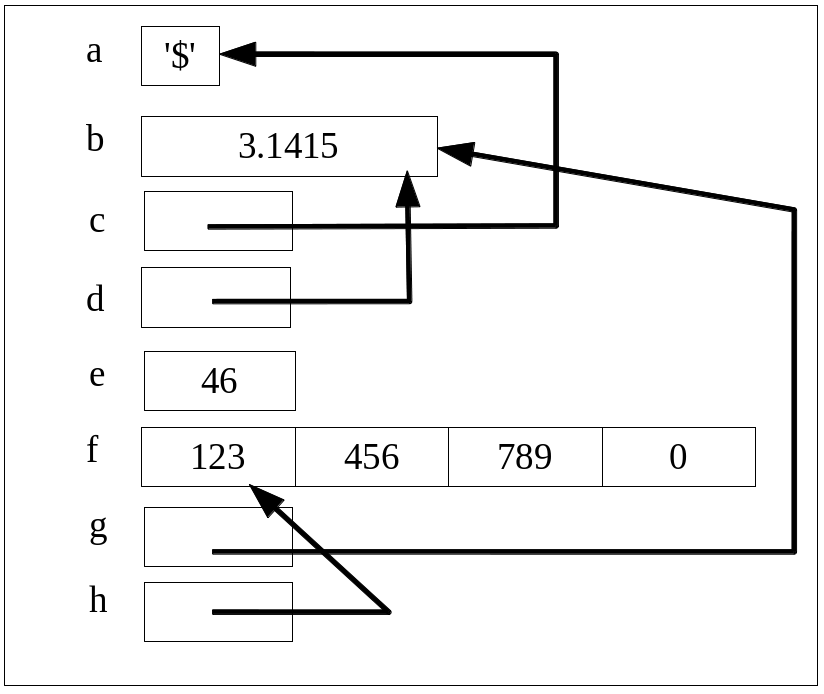
\includegraphics[width=3in]{pic2.PNG}
\end{center}
You noticed he was shaking his head as he walked away. Why?

\textsc{Answer:}
\begin{answercode}
d went from int pointer to double pointer
d and g are both pointing to b

\end{answercode}

%-------------------------------------------------------------------------------
\newpage
\nextq
The following program does compile and does run. But it has a memory leak.
Fix it so that there is no memory leak.

\textsc{Answer:}
\begin{answercode}
#include <iostream>

int sum(int n)
{
    int s = 0;
    int * i = new int;
    for (*i = 0; *i <= n; ++(*i))
    {
      s += *i;
    }
    delete i;
    return s;
}

int main()
{
    std::cout << sum(10) << '\n';
    return 0;
}
\end{answercode}

%-------------------------------------------------------------------------------
\newpage
\nextq
The following program get two integer values from the user 
and then prints the sum.
Do NOT use integer or double variables -- you can only use pointers.
In fact I have already declared all the variables you need,
i.e., two pointer variables.
You must allocate and deallocate memory correctly.

\textsc{Answer:}
\begin{answercode}
#include <iostream>

int main()
{
    int * p;
    int * q;

    // allocate memory for p
    int * p = new int;



    // allocate memory for q
    int *q = new int;

    // get integer value from user and store at integer that p points to
    std::cin >> *p;

    // get integer value from user and store at integer that q points to
    std::cin >> *q;

    // print the sum of integers that p and q point to
    std::cout << *p + *q << '\n';

    // deallocate memory used by q
    delete q;

    // deallcate memory used by p
    delete p;

    return 0;
}
\end{answercode}

%-------------------------------------------------------------------------------
\newpage
\nextq
Complete this code segment.

\textsc{Answer:}
\begin{answercode}
int x[] = {1, 5, 3, 7, 9, 4, 2, 6, 8, 0};
int max;

int * start = &x[0];
int * end = &x[10];
int * p;
int * pmax = &max;

// Complete the following to compute the maximum value in the array x
// from *start to *(end - 1) and store it in variable max.
// Your code must work for different array values in x.
// You also cannot use the name x or max.
// You must use a loop (of course).
// You can only use integer pointer variables start, end, p, pmax
void bubblesort(int * start,int  * end, int * p, int * pmax)
{
  *p = &x[0];
    for (int * p = end - 1; p >= start; --p)
    {
        for (int * q = start; q <= p; ++q)
        {
            if (*q > *(q + 1))
            {
                swap(*q, *(q + 1));
            }
        }
        if (*q > *p)
        {
          *pmax = *q;
        }
    }
}




// At this point the maximum value of *start,...,*(end - 1) is stored in
// variable max.
std::cout << max << '\n';
\end{answercode}

%-------------------------------------------------------------------------------
\newpage
\nextq
The following have a function that attempts to perform memory allocation
and memory deallocation, but
they are done incorrectly:
\vspace{-3mm}
\begin{Verbatim}[frame=single,fontsize=\small]
void mynew(int * p)
{
    p = new int;
}

void mydelete(int * p)
{
    delete p;
    p = NULL;
}

int main()
{
    int * p;
    mynew(p);
    *p = 42;
    mydelete(p);
    return 0;
}
\end{Verbatim}
\vspace{-5mm}Fix the above problem below.

\textsc{Answer:}\vspace{-3mm}
\begin{answercode}
void mynew(int *p)
{
  p = new int;
}

void mydelete(int * p)
{
  delete p;
}

int main()
{
    int * p;
    mynew(p);
    *p = 42;
    mydelete(p);
    return 0;
}
\end{answercode}

%-------------------------------------------------------------------------------
\newpage
\nextq
Complete the following by writing a struct and making any corrections.
\\
\textsc{Answer:}\vspace{-2mm}
\begin{answercode}
#include <iostream>

// define the struct here

struct student
{
  id = x.student_id;
  year = x.dob_year;
  month = x.dob_month;
  day = x.dob_day;
  height = x.height;
  weight = x.weight;
}



void input(Student * x)
{
    std::cin >> x.student_id; // get an integer value from user for x's 
                              // student id
    std::cin >> x.dob_year;   // get an integer value from user for x's year 
                              // of date of birth
    std::cin >> x.dob_month;  // get an integer value from user for x's month 
                              // of date of birth
    std::cin >> x.dob_day;    // get an integer value from user for x's day 
                              // of date of birth
    std::cin >> x.height;     // get a double value from user for x's height
    std::cin >> x.weight;     // get a double value frin user for x's weight
}

void print(Student & x)
{

  std::cout << student_id << ',' << student_year << ',' << student_month << ','
  << student_day << ',' << student_height << ',' << student_weight << '\n';




}

int main()
{
    Student john;
    input(john);
    println(john); // print all values of john separated by ',' and print '\n'
    return 0;
}
\end{answercode}

%-------------------------------------------------------------------------------
\newpage
\nextq
You are writing a tic-tac-toe game. The following code is in your
\verb!main()!:
\vspace{-3mm}
\begin{Verbatim}[frame=single,fontsize=\small]
#include <iostream>
#include "TTT.h"

int main()
{
    TTT board;

    while (1)
    {
        print(board);
        int row, col;
        get_input(board, row, col);
        make_move(board, row, col);
        if (game_ended(board)) 
        {
            break;
        }
    }
    print_result(board);

    return 0;
}
\end{Verbatim}
\vspace{-4mm}
Complete the header file (with the struct definition and the function
prototypes -- no function body definitions).
The struct and function prototypes must be minimal
(i.e., no useless member variables, no unnecessary parameters,
reference parameters must be constant whenever possible).

\textsc{Answer:}\vspace{-2mm}
\begin{answercode}
#ifndef TTT_H
#define TTT_H


  struct board
  {
   

    
  }















#endif
\end{answercode}

%-------------------------------------------------------------------------------
\newpage
\nextq
What is the output? Or is there an error?
\begin{Verbatim}[frame=single,fontsize=\small]
#include <iostream>

int h(int * p)
{
    return *p;
}

int * g(int * p)
{
    return p;
}

int * f(int * p)
{
    return (p != NULL ? g(p) : NULL);
}

int main()
{
    int i = 5;
    std::cout << *f(&i) + h(&i) << std::endl;
    return 0;
}
\end{Verbatim}

\textsc{Answer:}\vspace{-2mm}
\begin{answercode}
error because h is not a pointer


\end{answercode}

%-------------------------------------------------------------------------------
\newpage
\nextq
Complete the following program. Make sure there is no memory leak.

\textsc{Answer:}\vspace{-3mm}
\begin{answercode}
#include <iostream>

int f(int n)
{
    int * p;

    // Allocate an integer array of size n to p. (Of course the array
    // is in the heap.)
    int n [] = *p;





    // Fill the array that p points to with values 1, 2, 3, ..., n.
    for (int i = 0; i < 3; ++i)
    {
      n[] = i;
    }

    // Go over the values in the array that p points to and 
    // (1) if a value is odd, replace that value by the square root of the
    //     value, or
    if (n % 3 || n == 1)
    {
      n *= n;
    }
    
    // (2) if a value x is even, replace that value x by x + 1.
    else
    {
      n += 1;
    }
    // This is one pass.
    // Repeat this until every value in the array is <= 42.
    // Return the number of passes you have to run over the array

    int ret; // number of passes
    n = *p;
    int x = [n];
    for (int i = 0 ; i <=42; ++ i)
    {
      for (int i = 0; i < 3; ++i)
      {
        n[] = i;
      }
      if (n % 3 || n == 1)
      {
        n *= n;
      }
      else
      {
        n += 1;
      }
      ++ ret;
      
    }
    std::cout << ret << '\n';
    
















    
















    return ret;
}

int main()
{
    int n;
    std::cin >> n;
    std::cout << f(n) << '\n';
    return 0;
}
\end{answercode}

%-------------------------------------------------------------------------------
\newpage
\nextq
Complete the following function that performs the binary search.
You need NOT use recursion.
    
\textsc{Answer:}\vspace{-2mm}
\begin{answercode}
// Performs binary search on *start, *(start+1), ..., *(end - 1) for the
// value of target and return the pointer where target is found.
// If target is not found, NULL is returned.
int * binarysearch(int * start, int * end, int target)
{
  int * lower = start;
  int * upper = end - 1;
  while (lower <= upper)
  {
    int * mid = lower + (upper - lower) / 2;
        if (*mid == target)
        {
          return mid;
        }
        else if (target < *mid)
        {
          upper = mid - 1;
        }
        else
        {
          lower = mid + 1;
        }
  }
  return NULL;
}

\end{answercode}

%-------------------------------------------------------------------------------
\newpage
\nextq
Complete the program below. Here are two test cases.
\\
\textsc{Test 1}
\begin{console}[commandchars=\\\{\}]
\userinput{1 2 3}
\userinput{4 5 6}
4 5 6
1 2 3
\end{console}
\textsc{Test 2}
\begin{console}[commandchars=\\\{\}]
\userinput{10 9 8}
\userinput{5 6 7}
5 6 7
10 9 8
\end{console}

\textsc{Answer:}\vspace{-2mm}
\begin{answercode}
#include <iostream>

void swap(int ** p, int ** q))
{
    // You can only write at most 3 statements
    int t = &p;
    &p = &q ;
    &q = t

    return;
}

int main()
{
    int * p = new int[3];
    int * q = new int[3];
    for (int i = 0; i < 3; ++i)
    {
        std::cin >> p[i];
    }
    for (int i = 0; i < 3; ++i)
    {
        std::cin >> q[i];
    }

    swap(&p, &q);
    for (int i = 0; i < 3; ++i)
    {
        std::cout << p[i] << ' ';
    }
    std::cout << '\n';
    for (int i = 0; i < 3; ++i)
    {
        std::cin << q[i] << ' ';
    }
    std::cout << '\n';
    delete [] p;
    delete [] q;
    return 0;
}
\end{answercode}

%------------------------------------------------------------------------------
\newpage

\textsc{Instructions}

In \verb!main.tex! change the email address in
\begin{console}
\renewcommand\AUTHOR{jdoe5@cougars.ccis.edu} 
\end{console}
yours.
In the bash shell, execute \lq\lq \verb!make!" to recompile \verb!main.pdf!.
Execute \lq\lq \verb!make v!" to view \verb!main.pdf!.
Execute \lq\lq \verb!make s!" to create \verb!submit.tar.gz! for submission.

For each question, you'll see boxes for you to fill.
You write your answers in \verb!main.tex! file.
For small boxes, if you see
\begin{console}[frame=single=single,fontsize=\small]
1 + 1 = \answerbox{}.
\end{console}
you do this:
\begin{console}[frame=single=single,fontsize=\small]
1 + 1 = \answerbox{2}.
\end{console}
\verb!answerbox! will also appear in
\lq\lq true/false" and \lq\lq multiple-choice"
questions.

For longer answers that needs typewriter font, if you see
\begin{console}[frame=single=single, fontsize=\small]
Write a C++ statement that declares an integer variable name x.
\begin{answercode}
\end{answercode}
\end{console}
you do this:
\begin{console}[frame=single=single, fontsize=\small]
Write a C++ statement that declares an integer variable name x.
\begin{answercode}
int x;
\end{answercode}
\end{console}
\verb!answercode! will appear in questions asking for
code, algorithm, and program output.
In this case, indentation and spacing is significant.
For program output, I do look at spaces and newlines.

For long answers (not in typewriter font) if you see
\begin{console}[frame=single=single, fontsize=\small]
What is the color of the sky?
\begin{answerlong}
\end{answerlong}
\end{console}
you can write
\begin{console}[frame=single=single, fontsize=\small]
What is the color of the sky?
\begin{answerlong}
The color of the sky is blue.
\end{answerlong}
\end{console}
For students beyond 245: You can put \LaTeX\ commands in
\verb!answerbox! and 
\verb!answerlong!.

A question that begins with \lq\lq T or F or M"
requires you to identify whether it is true or
false, or meaningless.
\lq\lq Meaningless" means something's wrong with the statement and
it is not well-defined.
Something like \lq\lq $1 +_2$" or \lq\lq $\{2\}^{\{3\}}$" is not
well-defined.
Therefore a question such as
\lq\lq Is $42 = 1 +_2$ true or false?" or
\lq\lq Is $42 = \{2\}^{\{3\}}$ true or false?"
does not make sense.
\lq\lq Is $P(42) = \{42\}$ true or false?" is meaningless because $P(X)$
is only defined if $X$ is a set.
For \lq\lq Is 1 + 2 + 3 true or false?", \lq\lq 1 + 2 + 3" is well--defined but
as a
\lq\lq numerical expression", not as a \lq\lq proposition", i.e.,
it cannot be true or false.
Therefore \lq\lq Is 1 + 2 + 3 true or false?" is also not a well-defined
question.

When writing results of computations, make sure it's simplified.
For instance write $2$ instead of $1 + 1$.
When you write down sets,
if the answer is $\{1\}$, I do not
want to see $\{1, 1\}$.

When writing a counterexample, always write the simplest.

Here are some examples (see \verb!instructions.tex! for details):

\begin{enumerate}

 \item \tf: 1 + 1 = 2 \dotfill\answerbox{T}
 
 \item \tf: 1 + 1 = 3 \dotfill\answerbox{F}
 
 \item \tf: $1 +^2 =$ \dotfill\answerbox{M}
 
 \item $1 + 2 =$ \answerbox{3}
 
 \item Write a C++ statement to declare an integer variable named
 \verb!x!.
 \begin{answercode}
int x;
 \end{answercode}

 \item Solve $x^2 - 1 = 0$.
 \begin{answerlong}
 Since $x^2 - 1 = (x-1)(x+1)$, $x^2 - 1 = 0$ implies $(x-1)(x+1)=0$.
 Therefore $x - 1 = 0$ or $x = -1$.
 Hence $x = 1$ or $x = -1$.
 \end{answerlong}

 \item
 \begin{mcq}
 {Which is true?}{\answerbox{C}}
 {$1+1=0$}
 {$1+1=1$}
 {$1+1=2$}
 {$1+1=3$}
 {$1+1=4$}
 \end{mcq}


\end{enumerate}

\end{document}